\chapter{分形}
\label{chap:fractal}

\epigraph{一花一世界,一叶一菩提。}{《严华经》}

\section{无限长的曲线}
\label{sec:curve-with-infinite-length}

\subsection{科赫曲线}
\label{sec:Koch-curve}

将正三角形的每边三等分,以中间一分为边向外作正三角形。然后对得到的图形中的每边持续上述动作,可得到如下的一系列图形。若无限进行下去,则得到的曲线称为科赫曲线(Koch Curve)。

\def\kochsnowflake[#1,#2,#3]{%
  \coordinate(N1#1)at($2/3*(#2)+1/3*(#3)$);
  \coordinate(N2#1)at($1/3*(#2)+2/3*(#3)$);
  \coordinate(N3#1)at($(N2#1)!1!60:(N1#1)$);
  \ifnum#1=1
  \draw(#2)--(N1#1)--(N3#1)--(N2#1)--(#3);
  \else
  \ifnum#1=2
  \kochsnowflake[1,#2,  N1#1]
  \kochsnowflake[1,N1#1,N3#1]
  \kochsnowflake[1,N3#1,N2#1]
  \kochsnowflake[1,N2#1,#3]
  \else\ifnum#1=3
  \kochsnowflake[2,#2,  N1#1]
  \kochsnowflake[2,N1#1,N3#1]
  \kochsnowflake[2,N3#1,N2#1]
  \kochsnowflake[2,N2#1,#3]
  \else\ifnum#1=4
  \kochsnowflake[3,#2,  N1#1]
  \kochsnowflake[3,N1#1,N3#1]
  \kochsnowflake[3,N3#1,N2#1]
  \kochsnowflake[3,N2#1,#3]
  \else\ifnum#1=5
  \kochsnowflake[4,#2,  N1#1]
  \kochsnowflake[4,N1#1,N3#1]
  \kochsnowflake[4,N3#1,N2#1]
  \kochsnowflake[4,N2#1,#3]
  \else\ifnum#1=6
  \kochsnowflake[5,#2,  N1#1]
  \kochsnowflake[5,N1#1,N3#1]
  \kochsnowflake[5,N3#1,N2#1]
  \kochsnowflake[5,N2#1,#3]
  \fi\fi\fi\fi\fi
  \fi
}

\begin{center}
  \begin{tikzpicture}[scale=1.0]
    \begin{scope}
      \coordinate(A)at(0,0);\coordinate(B)at(2,0);\coordinate(C)at($(A)!1!60:(B)$);
      \draw(A)--(B)--(C)--cycle;
    \end{scope}
    \begin{scope}[shift={(2.5,0)}]
      \coordinate(A)at(0,0);\coordinate(B)at(2,0);\coordinate(C)at($(A)!1!60:(B)$);
      \coordinate(A1)at($2/3*(A)+1/3*(B)$);\coordinate(A2)at($1/3*(A)+2/3*(B)$);\coordinate(A3)at($(A2)!1!60:(A1)$);
      \coordinate(B1)at($2/3*(B)+1/3*(C)$);\coordinate(B2)at($1/3*(B)+2/3*(C)$);\coordinate(B3)at($(B2)!1!60:(B1)$);
      \coordinate(C1)at($2/3*(C)+1/3*(A)$);\coordinate(C2)at($1/3*(C)+2/3*(A)$);\coordinate(C3)at($(C2)!1!60:(C1)$);
      \draw(A)--(A1)--(A3)--(A2)--(B)--(B1)--(B3)--(B2)--(C)--(C1)--(C3)--(C2)--cycle;
      \draw[dashed](A1)--(A2) (B1)--(B2) (C1)--(C2);
    \end{scope}
    \begin{scope}[shift={(5,0)}]
      \coordinate(A)at(0,0);\coordinate(B)at(2,0);\coordinate(C)at($(A)!1!60:(B)$);
      \kochsnowflake[2,A,B]
      \kochsnowflake[2,B,C]
      \kochsnowflake[2,C,A]
    \end{scope}
    \begin{scope}[shift={(7.5,0)}]
      \coordinate(A)at(0,0);\coordinate(B)at(2,0);\coordinate(C)at($(A)!1!60:(B)$);
      \kochsnowflake[3,A,B]
      \kochsnowflake[3,B,C]
      \kochsnowflake[3,C,A]
    \end{scope}
    \begin{scope}[shift={(10,0)}]
      \coordinate(A)at(0,0);\coordinate(B)at(2,0);\coordinate(C)at($(A)!1!60:(B)$);
      \kochsnowflake[4,A,B]
      \kochsnowflake[4,B,C]
      \kochsnowflake[4,C,A]
    \end{scope}
  \end{tikzpicture}
\end{center}

% \begin{center}
%   \begin{tikzpicture}[scale=1.0]
%       \coordinate(A)at(0,0);\coordinate(B)at(4,0);\coordinate(C)at($(A)!1!60:(B)$);
%       \kochsnowflake[6,A,B]
%       \kochsnowflake[6,B,C]
%       \kochsnowflake[6,C,A]
%   \end{tikzpicture}
% \end{center}

显然,科赫曲线围成的面积是有限的,因为它位于某个圆内(请思考:是否位于初始正三角形的外接圆内?)。然而,其周长却是无限的。

\subsubsection{边}
\label{sec:koch-side}

显然,每个图形的边的数目数是前一图形边数的4倍\footnote{因为每条边变成4条边。},从而边数$s_n$可由下面公式给出:
\begin{align*}
  s_n=3\times 4^{n-1}
\end{align*}

同时可知边的长度是前一图形边的长度的$\frac13$。若记第一个正三角形的边长为$l$,则每个图形的边长$l_n$可由下式给出:
\begin{align*}
  l_n=\frac{l}{3^{n-1}}
\end{align*}

\subsubsection{周长}
\label{sec:koch-perimeter}

记第$n$个图形的周长是$P_n$,则容易知道
\begin{align*}
  P_{n+1} = \frac43\times P_n
\end{align*}
若假设初始正三角形的边长为1,则有$P_1=3$,从而有
\begin{align*}
  \lim_{n\to+\infty}P_n = \lim_{n\to+\infty}3\times\left(\frac43\right)^{n-1}=+\infty
\end{align*}
即面积有限的科赫曲线有无限长的周长\footnote{也可以由$P_n=s_n\times l_n$直接得到$P_n$的公式。}。

\subsubsection{面积}
\label{sec:koch-area}

第$n$个图形的面积比前一个图形多了$s_{n-1}$个小三角形,这些小三角形的边长为$l_n$,从而
\begin{align*}
  S_n = S_{n-1} + s_{n-1} \times \left(\frac{l_n}{l}\right)^2 \times S_1
\end{align*}


\section{二维}
\label{sec:2D-fractal}

\subsection{谢尔宾斯基三角形}
\label{sec:sierpinski-triangle}

\begin{center}
  \def\sierpinski[#1,#2,#3,#4]{
    \fill[color=black](#1)--(#2)--(#3)--cycle;
    \coordinate(N#1#2)at($0.5*(#1)+0.5*(#2)$);
    \coordinate(N#2#3)at($0.5*(#2)+0.5*(#3)$);
    \coordinate(N#3#1)at($0.5*(#3)+0.5*(#1)$);
    \fill[color=white](N#1#2)--(N#2#3)--(N#3#1)--cycle;
    \ifnum\numexpr#4>0
      \sierpinski[N#1#2,   #2,N#2#3,#4-1]
      \sierpinski[N#3#1,N#2#3,   #3,#4-1]
      \sierpinski[   #1,N#1#2,N#3#1,#4-1]
    \else
      
    \fi
  }
  \begin{tikzpicture}[scale=1.0]
    \begin{scope}[shift={(0,0)}]
      \coordinate(A)at(0,0);\coordinate(B)at(3,0);\coordinate(C)at($(A)!1!60:(B)$);
      \fill[color=black](A)--(B)--(C)--cycle;
    \end{scope}
    \begin{scope}[shift={(3.5,0)}]
      \coordinate(A)at(0,0);\coordinate(B)at(3,0);\coordinate(C)at($(A)!1!60:(B)$);
      \sierpinski[A,B,C,0]
    \end{scope}
    \begin{scope}[shift={(7,0)}]
      \coordinate(A)at(0,0);\coordinate(B)at(3,0);\coordinate(C)at($(A)!1!60:(B)$);
      \sierpinski[A,B,C,1]
    \end{scope}
    \begin{scope}[shift={(10.5,0)}]
      \coordinate(A)at(0,0);\coordinate(B)at(3,0);\coordinate(C)at($(A)!1!60:(B)$);
      \sierpinski[A,B,C,2]
    \end{scope}
    \begin{scope}[shift={(0,-3.5)}]
      \coordinate(A)at(0,0);\coordinate(B)at(3,0);\coordinate(C)at($(A)!1!60:(B)$);
      \sierpinski[A,B,C,3]
    \end{scope}
    \begin{scope}[shift={(3.5,-3.5)}]
      \coordinate(A)at(0,0);\coordinate(B)at(3,0);\coordinate(C)at($(A)!1!60:(B)$);
      \sierpinski[A,B,C,4]
    \end{scope}
    \begin{scope}[shift={(7,-3.5)}]
      \coordinate(A)at(0,0);\coordinate(B)at(3,0);\coordinate(C)at($(A)!1!60:(B)$);
      \sierpinski[A,B,C,5]
    \end{scope}
    \begin{scope}[shift={(10.5,-3.5)}]
      \coordinate(A)at(0,0);\coordinate(B)at(3,0);\coordinate(C)at($(A)!1!60:(B)$);
      \sierpinski[A,B,C,6]
    \end{scope}
  \end{tikzpicture}
\end{center}

如图,从一个黑色正三角形出发,每次从黑色三角形中扣出一个该黑色三角形的$\frac14$大小的正三角形,如此无限操作下去,就得到了谢尔宾斯基三角形(Sierpinski triangle,Sierpinski gasket,Sierpinski sieve)\footnote{波兰数学家Sierpiński在1915提出的,最早出现在13世纪的意大利艺术作品中。}。

记第一个三角形的边长为$L$,引入如下记号:
\begin{align*}
  N_n:{}&\text{第$n$个迭代后黑色三角形的个数}\\
  L_n:{}&\text{第$n$个迭代后黑色三角形的边长}\\
  A_n:{}&\text{第$n$个迭代后所有黑色三角形的总面积}
\end{align*}
其中第一个黑色三角形对应的$n=0$,由$N_n$和$L_n$都是等比数列容易得到以下关系:
\begin{align*}
  N_n={}& 3^n\\
  L_n={}& \left(\frac12\right)^n\cdot L=2^{-n}L\\
  A_n={}& N_n \cdot \left(\frac{\sqrt3}{4} L_n^2\right)=\frac{\sqrt3}{4} \left(\frac34\right)^n L^2
\end{align*}



\subsection{Sierpinski Carpet}
\label{sec:sierpinski-carpet}

\begin{center}
  % https://tex.stackexchange.com/questions/341791/generating-a-sierpinski-carpet-with-tikz
  \newcount\sierpinskiorder
  \newcommand\sierpinskicarpet[2][]{%
    \tikzset{sierpinski/.cd,#1}%
    \sierpinskiorder=#2\relax%
    \path [sierpinski/background/.try] (0,0) rectangle (1,1);
    \SierpinskiCarpet}
  \def\SierpinskiCarpet{{%
      \ifnum\sierpinskiorder>0\relax
      \path [sierpinski/foreground/.try] (1/3, 1/3) rectangle ++(1/3, 1/3);
      \advance\sierpinskiorder by -1\relax
      \foreach \x in {0,...,2}{\foreach \y in {0,...,2}{
          \begin{scope}[shift={(\x/3,\y/3)},scale=1/3]
            \SierpinskiCarpet
          \end{scope}
        }}
      \fi
    }}
  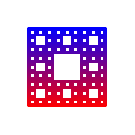
\begin{tikzpicture}
    \sierpinskicarpet[foreground/.style={fill=white},
    background/.style={top color=blue, bottom color=red}]{3}
  \end{tikzpicture}
  % \def\sierpinskiblanket[#1,#2,#3,#4,#5]{
  %   \fill[color=white](#1)--(#2)--(#3)--(#4)--cycle;

  %   \coordinate(N1#1)at(#1);
  %   \coordinate(N2#1)at($2/3*(#1)+1/3*(#2)$);
  %   \coordinate(N3#1)at($1/3*(#1)+2/3*(#2)$);
  %   \coordinate(N4#1)at(#2);

  %   \coordinate(N5#1)at($2/3*(#1)+1/3*(#4)$);
  %   \coordinate(N6#1)at($2/3*(#1)+1/3*(#3)$);
  %   \coordinate(N7#1)at($2/3*(#2)+1/3*(#4)$);
  %   \coordinate(N8#1)at($2/3*(#2)+1/3*(#3)$);

  %   \coordinate(N9#1) at($2/3*(#4)+1/3*(#1)$);
  %   \coordinate(N10#1)at($2/3*(#4)+1/3*(#2)$);
  %   \coordinate(N11#1)at($2/3*(#3)+1/3*(#1)$);
  %   \coordinate(N12#1)at($2/3*(#3)+1/3*(#2)$);

  %   \coordinate(N13#1)at(#4);
  %   \coordinate(N14#1)at($2/3*(#4)+1/3*(#3)$);
  %   \coordinate(N15#1)at($2/3*(#3)+1/3*(#4)$);
  %   \coordinate(N16#1)at(#3);
    
  %   \fill[color=black](N6#1)--(N7#1)--(N11#1)--(N10#1)--cycle;

  %   \ifnum\numexpr#5>0
  %     \sierpinskiblanket[N1#1,N2#1,N6#1,N5#1,#5-1]
  %     \sierpinskiblanket[N2#1,N3#1,N7#1,N6#1,#5-1]
  %     \sierpinskiblanket[N3#1,N4#1,N8#1,N7#1,#5-1]
  %     \sierpinskiblanket[N5#1,N6#1,N10#1,N9#1,#5-1]
  %     \sierpinskiblanket[N7#1,N8#1,N12#1,N11#1,#5-1]
  %     \sierpinskiblanket[N9#1,N10#1,N14#1,N13#1,#5-1]
  %     \sierpinskiblanket[N10#1,N11#1,N15#1,N14#1,#5-1]
  %     \sierpinskiblanket[N11#1,N12#1,N16#1,N15#1,#5-1]
  %     \fi
  % }
  % \begin{tikzpicture}[scale=1.0]
  %   \coordinate(A)at(0,0);\coordinate(B)at(4,0);\coordinate(C)at(4,4);\coordinate(D)at(0,4);
  %   \draw(A)--(B)--(C)--(D)--cycle;
  %   \sierpinskiblanket[A,B,C,D,2]
  % \end{tikzpicture}
\end{center}

\subsection{Vicsek雪花}
\label{sec:vicsek-fractal}

\begin{center}
  \def\vicsek[#1,#2,#3]{
    \coordinate(N0#1#2)at(#1 |- #2);
    \coordinate(N9#1#2)at(#1 -| #2);

    \coordinate(N1#1#2)at(#1);
    \coordinate(N2#1#2)at($2/3*(#1)+1/3*(#2)$);
    \coordinate(N3#1#2)at($1/3*(#1)+2/3*(#2)$);
    \coordinate(N4#1#2)at(#2);
    \coordinate(N5#1#2)at($1/3*(#1)+2/3*(N0#1#2)$);
    \coordinate(N6#1#2)at($1/3*(#2)+2/3*(N0#1#2)$);
    \coordinate(N7#1#2)at($1/3*(#1)+2/3*(N9#1#2)$);
    \coordinate(N8#1#2)at($1/3*(#2)+2/3*(N9#1#2)$);
    \ifnum\numexpr#3>0
      \vicsek[N1#1#2,N2#1#2,#3-1]
      \vicsek[N2#1#2,N3#1#2,#3-1]
      \vicsek[N3#1#2,N4#1#2,#3-1]
      \vicsek[N5#1#2,N6#1#2,#3-1]
      \vicsek[N7#1#2,N8#1#2,#3-1]
    \else
      \fill[color=black](N1#1#2)rectangle(N2#1#2);
      \fill[color=black](N2#1#2)rectangle(N3#1#2);
      \fill[color=black](N3#1#2)rectangle(N4#1#2);
      \fill[color=black](N5#1#2)rectangle(N6#1#2);
      \fill[color=black](N7#1#2)rectangle(N8#1#2);
    \fi
  }
  \begin{tikzpicture}[scale=.8]
    \begin{scope}[shift={(0,0)}]
      \coordinate(A)at(0,0);\coordinate(B)at(3,3);
      \vicsek[A,B,0]
    \end{scope}
    \begin{scope}[shift={(4,0)}]
      \coordinate(A)at(0,0);\coordinate(B)at(3,3);
      \vicsek[A,B,1]
    \end{scope}
    \begin{scope}[shift={(8,0)}]
      \coordinate(A)at(0,0);\coordinate(B)at(3,3);
      \vicsek[A,B,2]
    \end{scope}
    \begin{scope}[shift={(12,0)}]
      \coordinate(A)at(0,0);\coordinate(B)at(3,3);
      \vicsek[A,B,3]
    \end{scope}
    % \begin{scope}[shift={(16,0)}]
    %   \coordinate(A)at(0,0);\coordinate(B)at(3,3);
    %   \vicsek[A,B,4] %% Recursion exceeds the capacity of TeX!!
    % \end{scope}
  \end{tikzpicture}
\end{center}


\section{设计分形}
\label{sec:designing-fractal}

以一个图形为基础,按一定的规律做迭代,可有望得到一个分形。

\begin{example}
  以正方形为基础,与Koch snowflake类似,每边向外凸出一个小正方形。
  \begin{center}
    \def\squarefractalline[#1,#2,#3]{
      \coordinate(N1#1#2)at($2/3*(#1)+1/3*(#2)$);
      \coordinate(N4#1#2)at($1/3*(#1)+2/3*(#2)$);
      \coordinate(N2#1#2)at($(N1#1#2)!1!-90:(N4#1#2)$);
      \coordinate(N3#1#2)at($(N2#1#2)+(N4#1#2)-(N1#1#2)$);

      \ifnum\numexpr#3>0
        \draw(#1)--(N1#1#2);
        \draw(N4#1#2)--(#2);
        \squarefractalline[N1#1#2,N2#1#2,#3-1]
        \squarefractalline[N2#1#2,N3#1#2,#3-1]
        \squarefractalline[N3#1#2,N4#1#2,#3-1]
      \else
        \draw(#1)--(N1#1#2)--(N2#1#2)--(N3#1#2)--(N4#1#2)--(#2);
      \fi
    }
    \def\squarefractal[#1,#2,#3,#4,#5]{
      \squarefractalline[#1,#2,#5]
      \squarefractalline[#2,#3,#5]
      \squarefractalline[#3,#4,#5]
      \squarefractalline[#4,#1,#5]
    }
    \begin{tikzpicture}[scale=1.0]
      \begin{scope}[shift={(0,0)}]
        \coordinate(A)at(0,0);\coordinate(B)at(3,0);\coordinate(C)at(3,3);\coordinate(D)at(0,3);
        \draw(A)--(B)--(C)--(D)--cycle;
        % \squarefractalline[A,B,3]
      \end{scope}
      \begin{scope}[shift={(7,0)}]
        \coordinate(A)at(0,0);\coordinate(B)at(3,0);\coordinate(C)at(3,3);\coordinate(D)at(0,3);
        \squarefractal[A,B,C,D,1]
      \end{scope}
      \begin{scope}[shift={(0,-7)}]
        \coordinate(A)at(0,0);\coordinate(B)at(3,0);\coordinate(C)at(3,3);\coordinate(D)at(0,3);
        \squarefractal[A,B,C,D,2]
      \end{scope}
      \begin{scope}[shift={(7,-7)}]
        \coordinate(A)at(0,0);\coordinate(B)at(3,0);\coordinate(C)at(3,3);\coordinate(D)at(0,3);
        \squarefractal[A,B,C,D,3]
      \end{scope}
    \end{tikzpicture}
  \end{center}
\end{example}
